Milestones:
\begin{table}[H]
\caption{Dates of expected and actual progress}
\centering
\begin{tabular}{ccc}
\toprule
Milestones & Expected & Actual\\
\midrule
Template & 28.Nov.2019 & 25.Nov.2019\\
Distribution of different tasks (CEO,...) & 04.Dez.2019 &04.Dez.2019\\
Outline & 11.Dez.2019& 18.Dez.2019\\
Splitting up specific topics & 11.Dez.2019&12.Dez.2019\\
Section IV & 04.Jan.2020&09.Jan.2020\\
Paper finished& 23.Jan.2020& 30.Jan.2020\\
Presentation & 30.Jan.2020& \\
\bottomrule
\end{tabular}
\end{table}
The expected progress for this paper was mostly adhered to which can be seen in figure 1. \\
The specific dates are displayed in table 5.\\
Some self-imposed deadlines were exceeded, but never more than a week or than the appointed deadlines in class. As a group we managed to dispense the workload equally for all team members. We met 4 times, which helped immensely to solve any difficulties or questions. 

\begin{figure}[H]
\centering
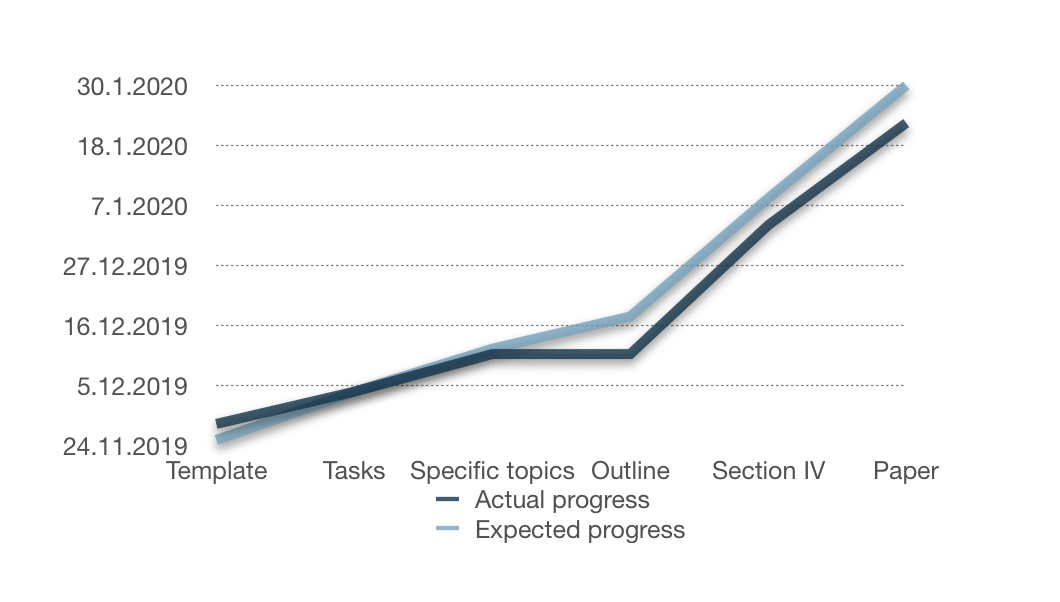
\includegraphics[scale=0.5]{Progress_chart}
\caption{Progress chart}
\end{figure}

